\documentclass[../AnalysisNoteJBuxton.tex]{subfiles}
\begin{document}

\subsection{Typical Correlation Function Construction}
\label{TypicalCfConstruction}

Typically, in practice, $B(k^{*})$ is obtained by forming mixed-event pairs, i.e. particles from a given event are paired with particles from N$_{mix}$(= 5) other events, and these pairs are then binned in $k^{*}$.
In forming the background distribution, it is important to mix only similar events; mixing events with different phase-spaces can lead to artificial signals in the correlaton function.
Therefore, in this analysis, we mix events with primary vertices within 2 cm and centralities within 5\% of each other.
Also note, a vertex correction is also applied to each event, which essentially recenters the the primary vertices to z = 0.

Figures \ref{fig:AllCfs:a}, \ref{fig:AllCfs:b}, \ref{fig:AllCfs:c} show the correlation functions for all centalities studied for \LamKchPALamKchM, \LamKchMALamKchP, and \LamALamKs, respectively. All were normalized in the range 0.32 $< k^{*} < $ 0.4 GeV/c.

\begin{figure}[h!]
  \centering
  %%----start of first subfigure---  
  \subfloat[\LamKchP (left) and \ALamKchM (right) correlations for 0-10\% (top), 10-30\%(middle), and 30-50\%(bottom) centralities.]{
    \label{fig:AllCfs:a}
    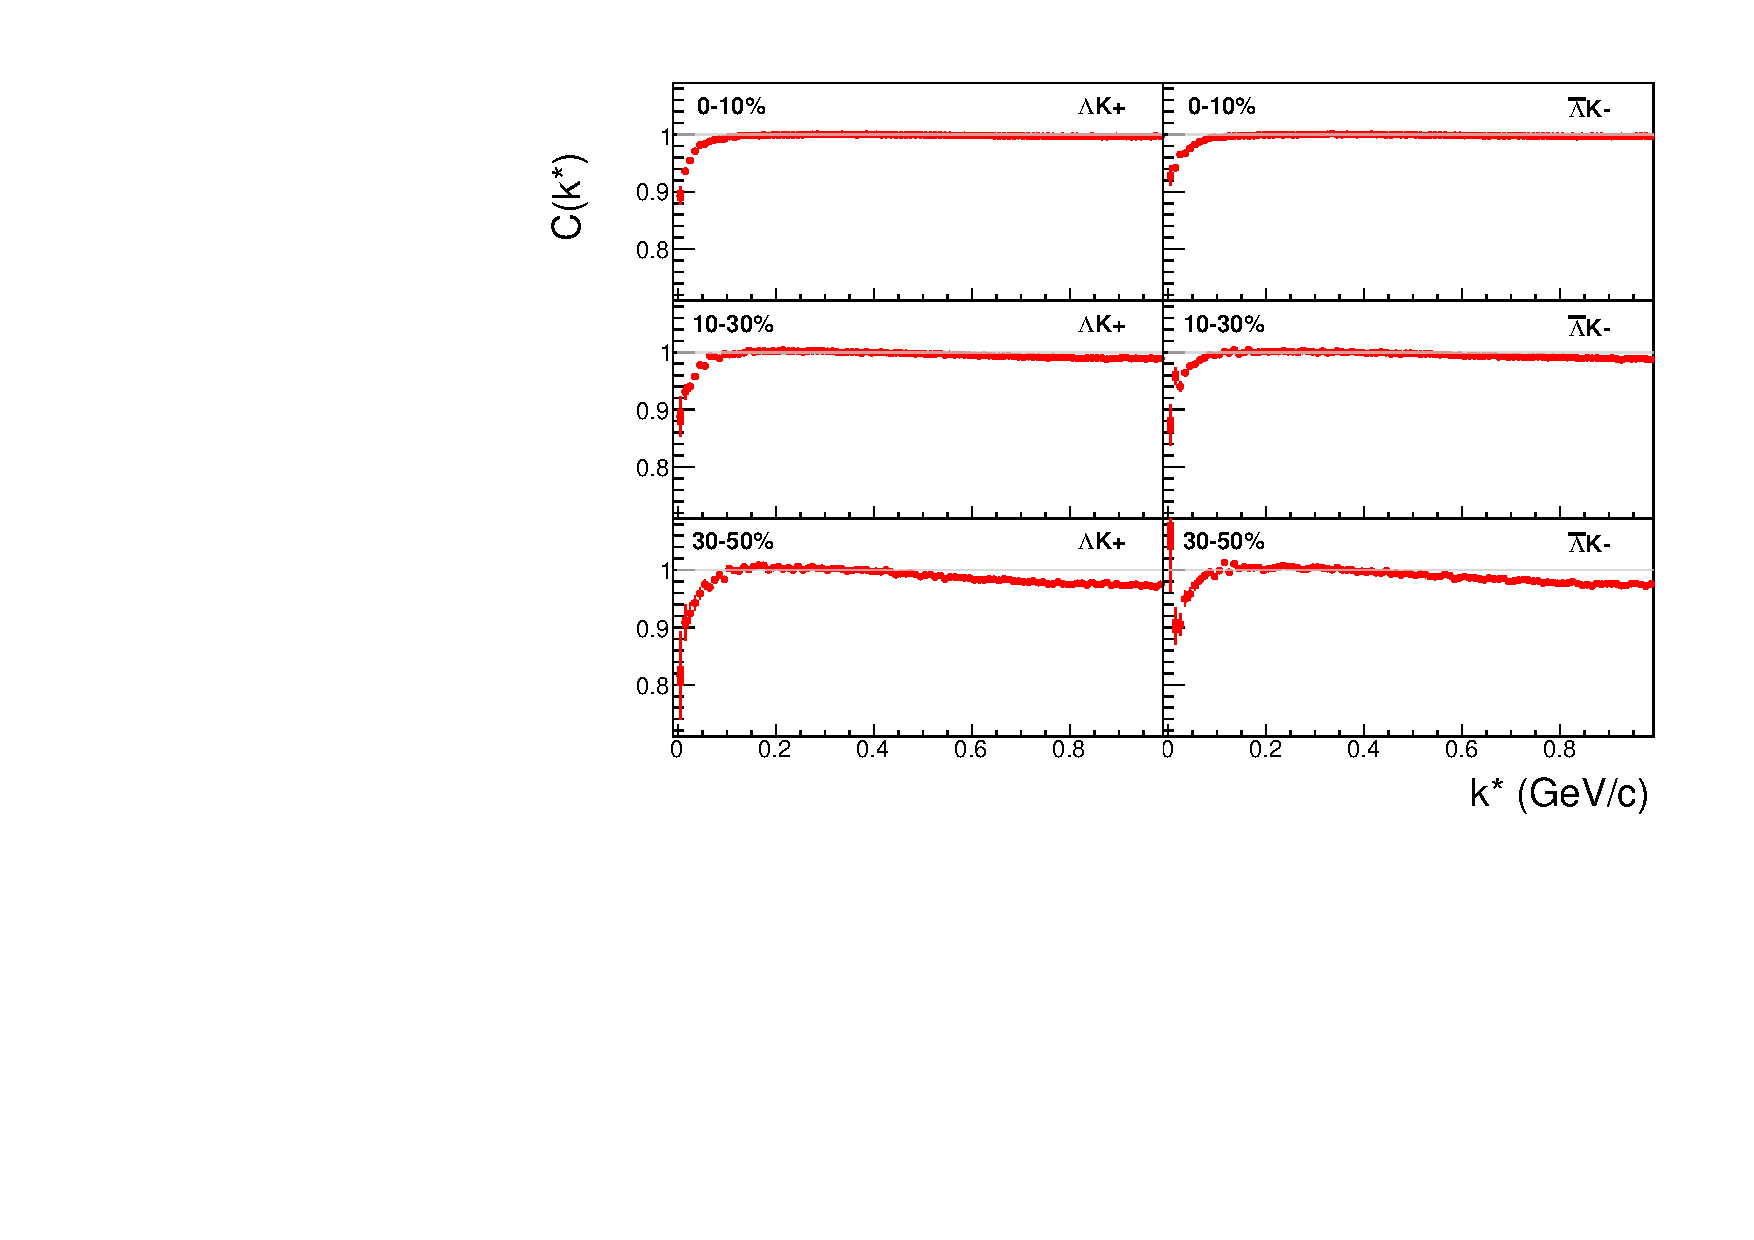
\includegraphics[width=0.49\textwidth]{4_CorrelationFunctions/Figures/canKStarCfsLamKchPwConj_0010_1030_3050.pdf}}
  %%----start of second subfigure---
  \subfloat[\LamKchM (left) and \ALamKchP (right) correlations for 0-10\% (top), 10-30\%(middle), and 30-50\%(bottom) centralities.  The peak at k* $\approx$ 0.2 GeV/c is due to the $\Omega^{-}$ resonance.]{
    \label{fig:AllCfs:b}
    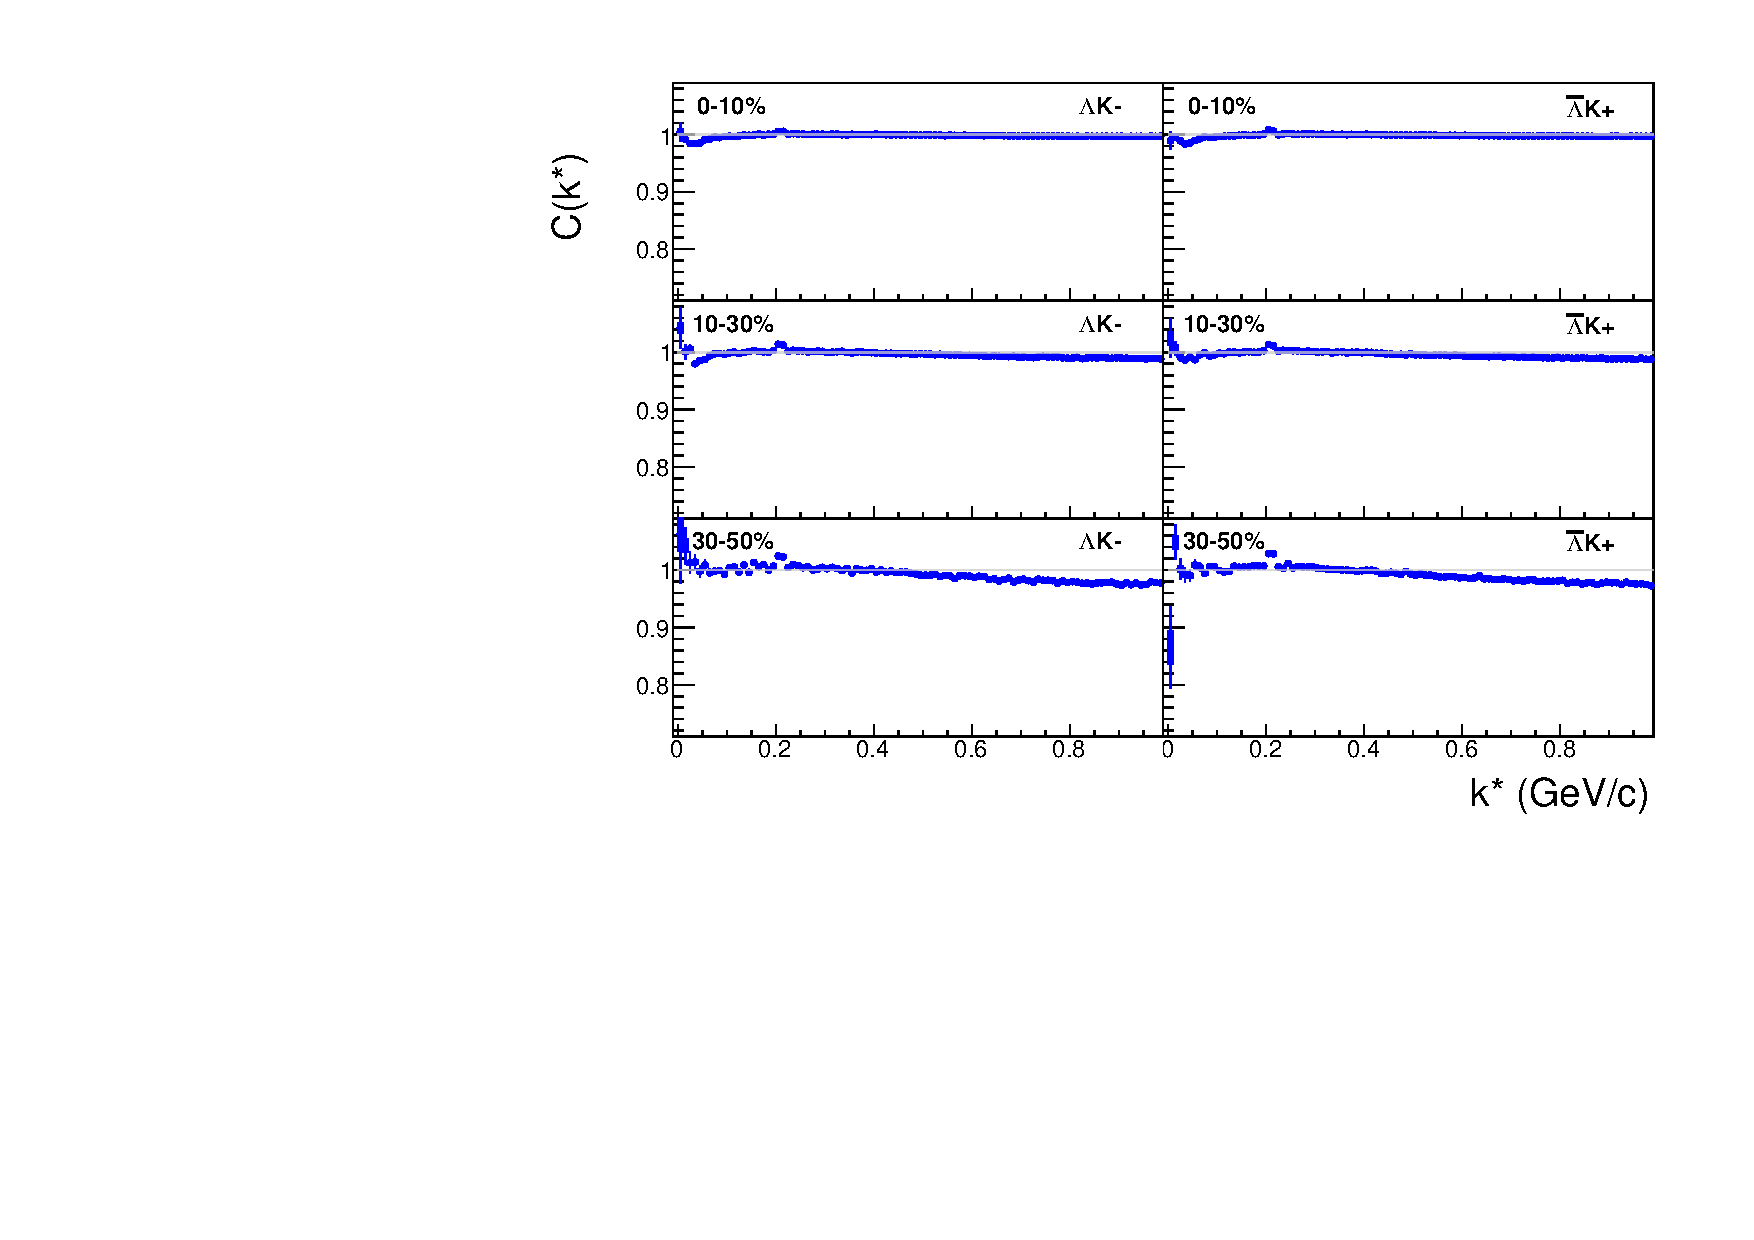
\includegraphics[width=0.49\textwidth]{4_CorrelationFunctions/Figures/canKStarCfsLamKchMwConj_0010_1030_3050.pdf}}
  \\  
  %%----start of third subfigure---
  \subfloat[\LamKs (left) and \ALamKs (right) correlations for 0-10\% (top), 10-30\%(middle), and 30-50\%(bottom) centralities.]{
    \label{fig:AllCfs:c}
    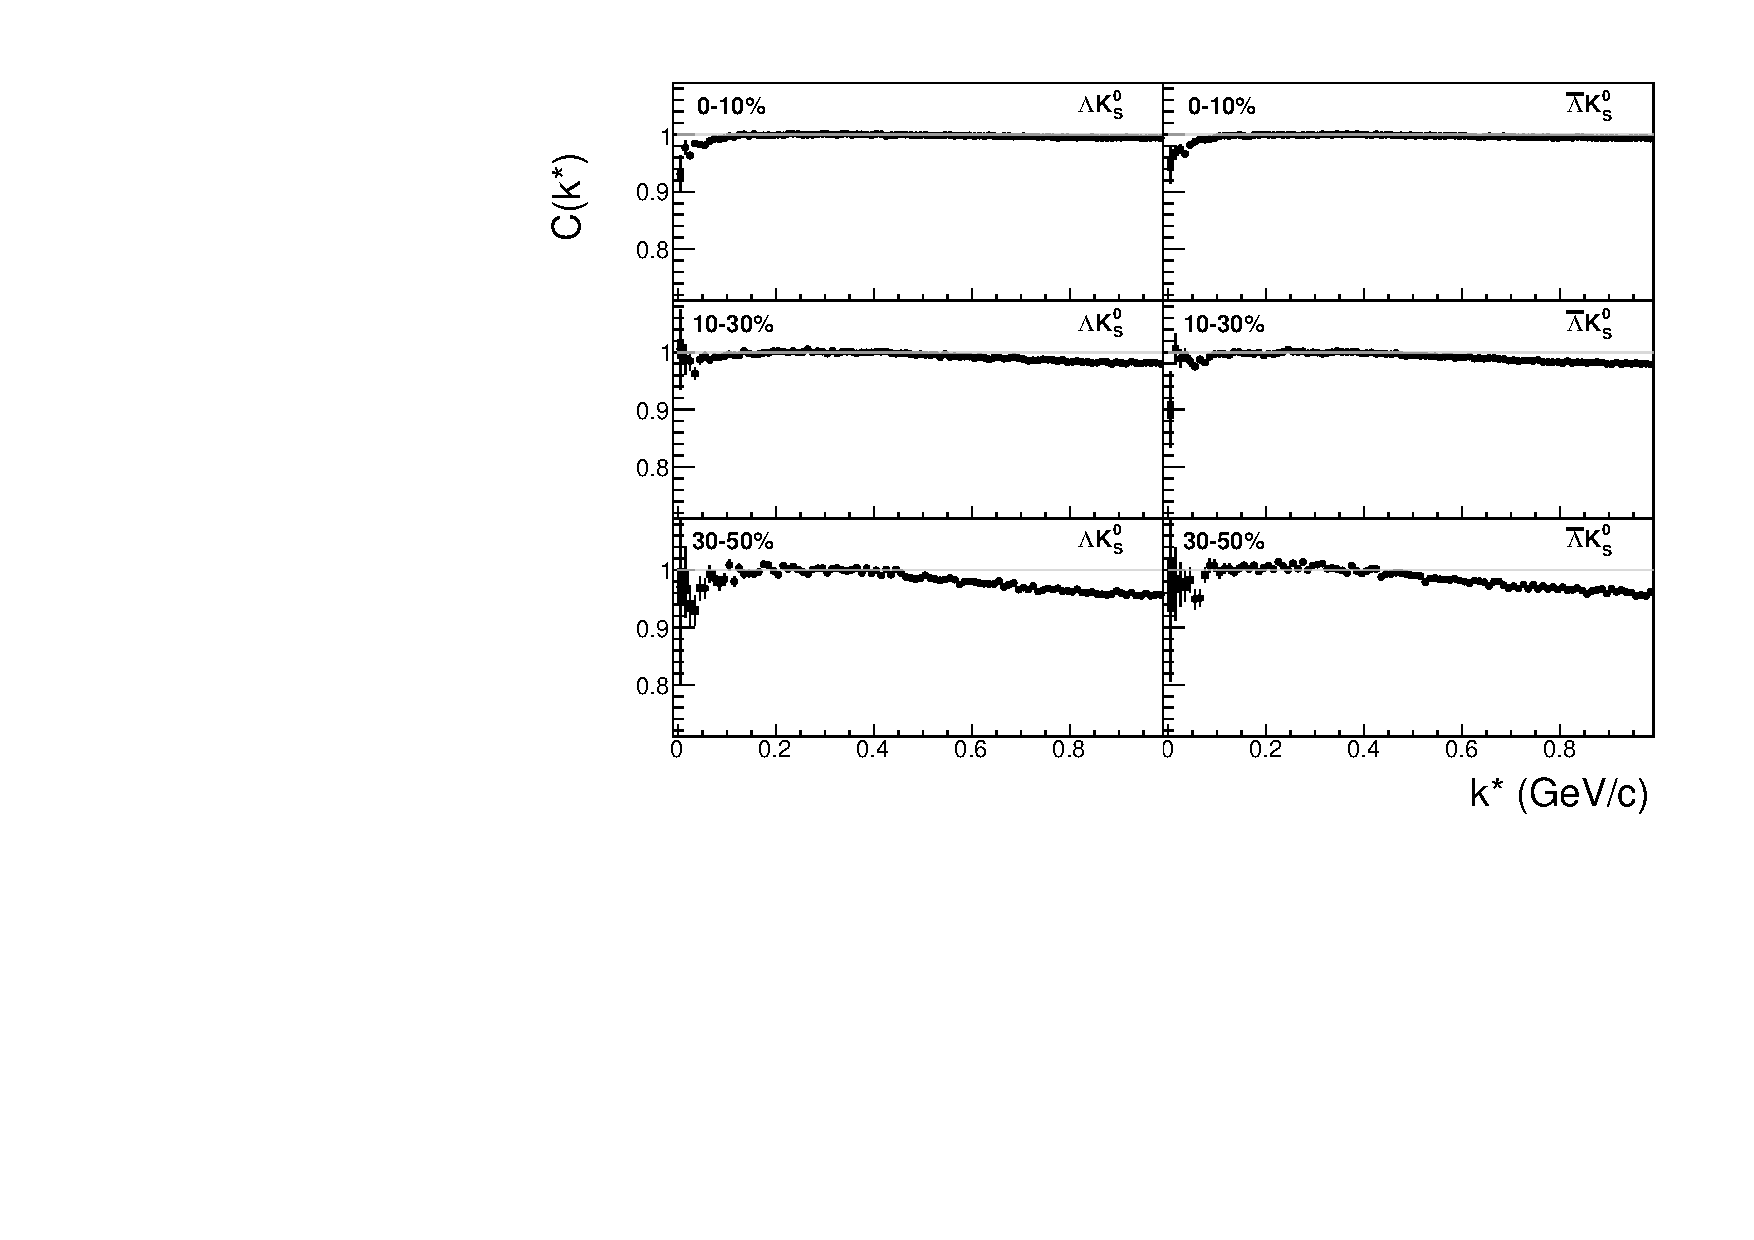
\includegraphics[width=0.49\textwidth]{4_CorrelationFunctions/Figures/canKStarCfsLamK0wConj_0010_1030_3050.pdf}}    
  %%----overall caption----
  \caption[\LamK Correlation Functions]{\LamK and \ALamAK correlation functions for 0-10\%, 10-30\%, and 30-50\% centralities.  The lines represent the statistical errors, while the boxes represent the systematic errors.}
  \label{fig:AllCfs}
\end{figure}


\begin{figure}[h]
  \centering
  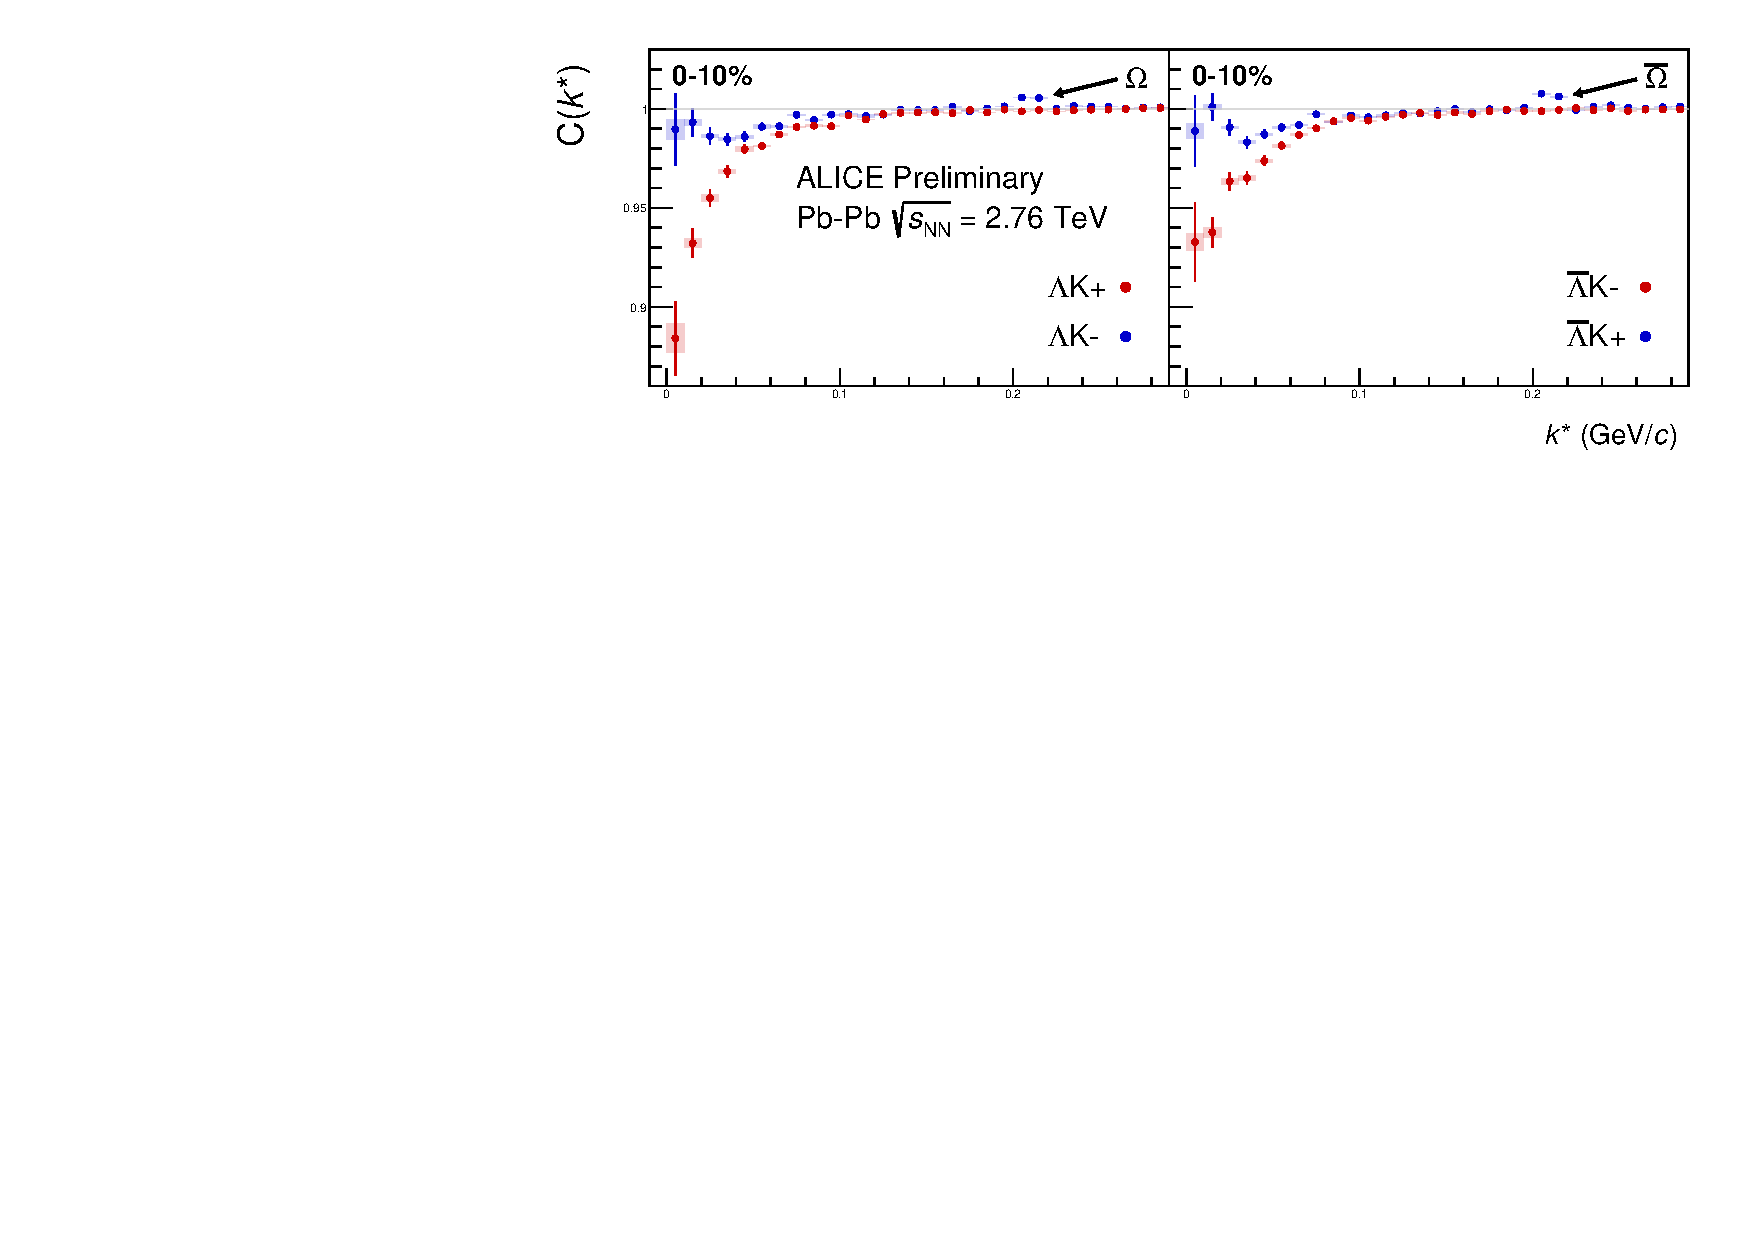
\includegraphics[width=\textwidth]{4_CorrelationFunctions/Figures/canLamKchPvsLamKchM0010.pdf}
  \caption[Correlation Functions: $\Lambda$K$^{+}$ vs $\Lambda$K$^{-}$ for 0-10\% Centrality]{Correlation Functions: $\Lambda$K$^{+}$ vs $\Lambda$K$^{-}$ ($\bar{\Lambda}$K$^{+}$ vs $\bar{\Lambda}$K$^{-}$) for 0-10\% centrality.  The peak in $\Lambda$K$^{-}$($\bar{\Lambda}$K$^{+}$) at k* $\approx$ 0.2 GeV/c is due to the $\Omega^{-}$ resonance.  The lines represent the statistical errors. (NOTE: This figure is slightly dated, and a new one will be generated which includes both statistical and systematic uncertainties)}
  \label{fig:cLamcKchCfs0010}
\end{figure}

\clearpage

\end{document}